\documentclass[11pt]{article}

\newcommand{\cnum}{CM146}
\newcommand{\ced}{Fall 2018}
\newcommand{\ctitle}[3]{\title{\vspace{-0.5in}\cnum, \ced\\Problem Set #1: #2}}
\usepackage{enumitem}
\newcommand{\solution}[1]{{{\color{blue}{\bf Solution:} {#1}}}}
\usepackage[usenames,dvipsnames,svgnames,table,hyperref]{xcolor}
\usepackage{graphicx}
\graphicspath{ {./images/} }
\usepackage{amsmath}
\usepackage{amssymb}

\renewcommand*{\theenumi}{\alph{enumi}}
\renewcommand*\labelenumi{(\theenumi)}
\renewcommand*{\theenumii}{\roman{enumii}}
\renewcommand*\labelenumii{\theenumii.}


\begin{document}
\title{CM146, Fall 2018 \\ Problem Set 1: Decision Trees and KNN}
\author{Gajan Nagaraj}
\date{10/29/2018}
\maketitle
\vspace{-0.75in}

\section{Problem 1}
Submitted on online CCLE quiz.

\newpage
\section{Problem 2}

\solution{}\\
The solution to this problem is justified logically as such: \\
We split our examples into $k$ disjoint subsets, each with ratio of $\frac{p_{k}}{p_{k}+n_{k}}$. Because each $k$ has the same ratio, our entropy will be the same regardless of the $S_{k}$ subset chosen. Thus we have no information gain for $S$. \\
The mathematical proof of this is as follows: \\
We know that the formula to calculate information gain is: \\
\centerline{$Gain(S,A) = Entropy(S) - \sum_{v \in Values(A)} \frac{S_{v}}{S} Entropy(S_{v})$} \\
We also know that the entropy of $S$ is defined as: \\
\centerline{$Entropy(S) = B(\frac{p}{p+n})$} \\
Substituting all these values into the Gain equation gives us: \\
\centerline{$Gain(S,A) = B(\frac{p}{p+n}) - B(\frac{p_{k}}{p_{k}+n_{k}})$} \\
We know that $S$ is made up of $k$ subsets with ratio $\frac{p_{k}}{p_{k}+n_{k}}$. Thus, $S$ itself must have ratio of $\frac{p_{k}}{p_{k}+n_{k}}$. \\
We can conclude that: \\
\centerline{$B(\frac{p}{p+n}) = B(\frac{p_{k}}{p_{k}+n_{k}})$} \\
\boxed{\therefore Gain = 0}

\newpage

\section{Problem 3}
\begin{enumerate}
\item Problem 3a \\
\solution{}
A $k=1$ would minimize the training set error for this data set. This is because the problem specified that each point can be its own neighbor. Thus if we can classify the point with its own label, then we will never have an error. With a $k=1$ and the fact that each point can be its own neighbor than we can conclude that if we check a point against itself we will have no training error, because a point will be labeled as it actually is. Each point will be labeled with 100\% accuracy. 
\item Problem 3b \\
\solution{}
Too small value of $k$ would result in overfitting. If we bias the model towards the training data, then we will have a lower chance of predicting the labels of a test data set that the model has not seen before. Additionally, a small $k$ would result in each point being overly influenced by its direct neighbor. Too large of a $k$ would introduce too much noise into the system because we would take into account features of unrelated neighbors that are located too far away. This would result in incorrect data classification.
\item Problem 3c \\
\solution{}
The value of $k$ that minimizes leave on out cross validation error for this data set is $k=5$. If we observe the data set, we can see that the only four points that can be classified incorrectly are isolated positive and negative signs on the opposing sides of the graph. The labels for these four points will be incorrectly computed as a result of the opposite signs around them. If we set our $k=5$, then we will only guess these four points incorrectly. This will result in an error of $\frac{4}{14}=\frac{2}{7}$.
\end{enumerate}
\newpage

\section{Problem 4}
\begin{enumerate}
\item Problem 4a \\
\solution{} \\
Person Class: \\
\centerline{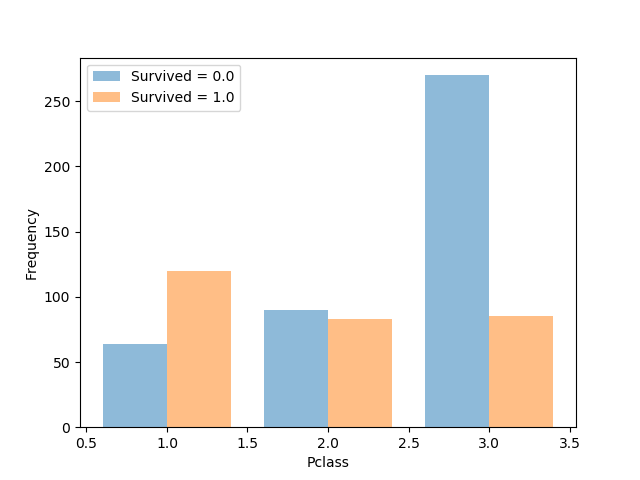
\includegraphics[scale=0.5]{1}} \\
Ratio of dead to survive increased as class number increased. \\ 
Sex: \\
\centerline{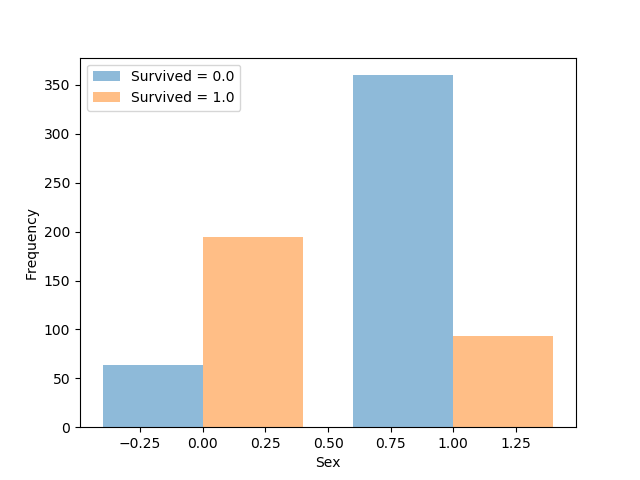
\includegraphics[scale=0.5]{2}} \\ 
Sex0 more survived than died. Sex1 much more died than survived. \\
\newpage
Age: \\ 
\centerline{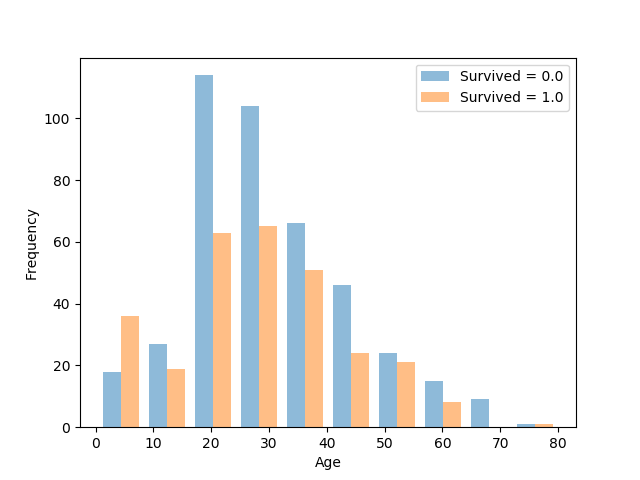
\includegraphics[scale=0.5]{3}} \\
Only ages 0-10 had more people survive than die. Ages 70-80 was close to this as well. Every other age range had more people die than survive.\\
Sibling/Spouse: \\
\centerline{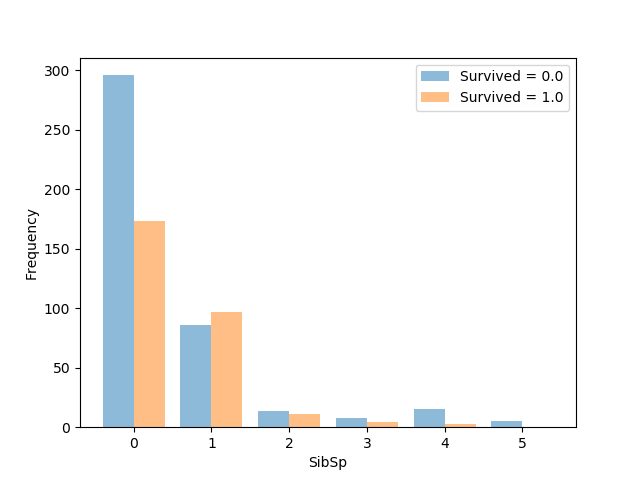
\includegraphics[scale=0.5]{4}} \\
Those who did not have siblings/spouse on board were much more likely to die. 1-2 siblings/spouse produced the best chance of survival. \\
\newpage
Parents/Children: \\
\centerline{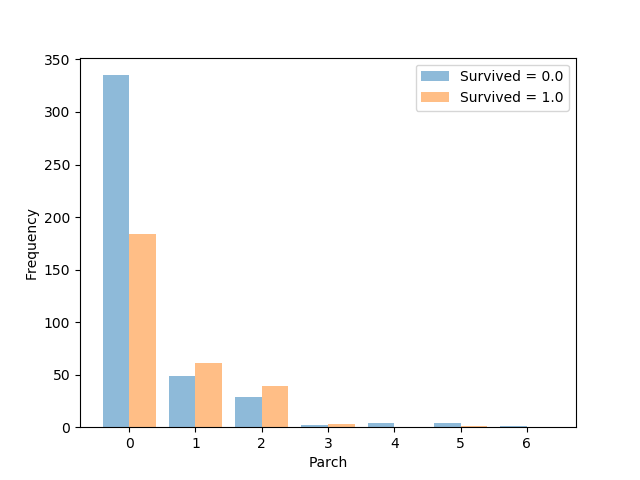
\includegraphics[scale=0.5]{5}} \\
Those with no parents/children or too many parents/children were likely to die. 1-3 parents/children produced the best chance of survival. \\
Fare: \\
\centerline{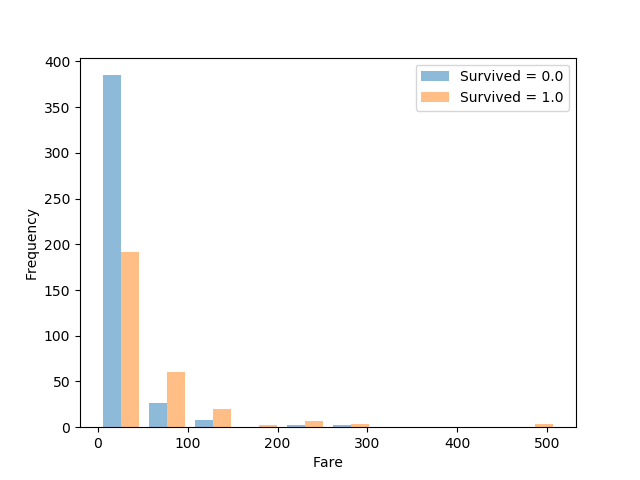
\includegraphics[scale=0.5]{6}} \\
The higher the fare one paid, the more likely survival was. \\
\newpage
Embarked: \\
\centerline{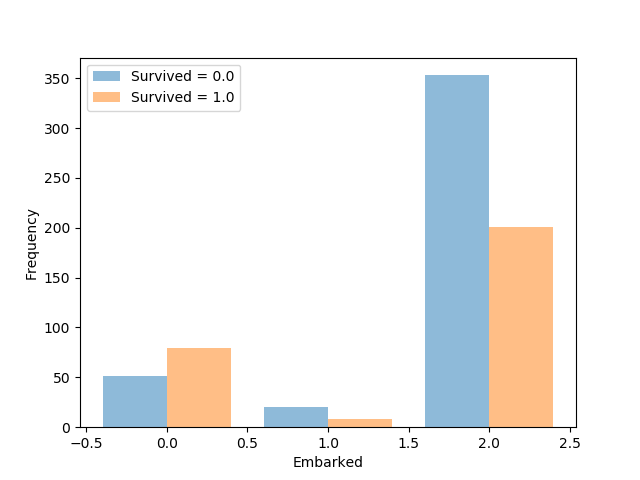
\includegraphics[scale=0.5]{7}} \\
Those who embarked from port0 were more likely to survive than die.

\item Problem 4b \\
\solution{} \\
I implemented the RandomClassifier and obtained an error of 0.485. I also observed that this error is higher than that obtained from the MajorityVoteClassifier.

\item Problem 4c \\
\solution{} \\
The training error I got for the DecisionTreeClassifier is 0.014.

\item Problem 4d \\
\solution{} \\
The training error I got for the KNeighborsClassifier for: \\
$k = 3 \rightarrow 0.167$ \\
$k = 5 \rightarrow  0.201$ \\
$k = 7 \rightarrow  0.240$ \\

\item Problem 4e \\
\solution{} \\
Below is the training and testing error of each of the classifiers: \\
Classifying using Majority Vote: 
\begin{itemize}
	\item training error: 0.404
	\item testing error: 0.407
\end{itemize}
Classifying using Random: 
\begin{itemize}
	\item training error: 0.489
	\item testing error: 0.487
\end{itemize}
Classifying using Decision Tree: 
\begin{itemize}
	\item training error: 0.012
	\item testing error: 0.241
\end{itemize}
Classifying using k-Nearest Neighbors (k=5): 
\begin{itemize}
	\item training error: 0.212
	\item testing error: 0.315
\end{itemize}

\item Problem 4f \\
\solution{} \\
The following graph of $k$ vs validation error was generated from the code: \\
\centerline{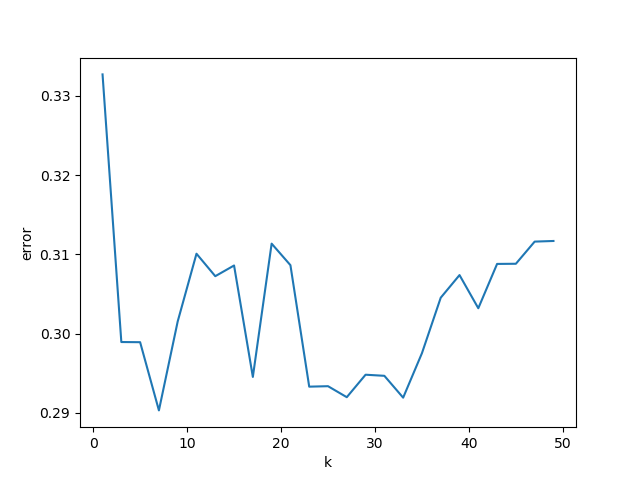
\includegraphics[scale=0.5]{Figure_1}}
A value of k = 7 yields the least validation error. Additionally, I noticed that the validation error decreased when increasing k from 0 to 7, but increases after.

\item Problem 4g \\
\solution{} \\
From the code, I obtained the following graph: \\
\centerline{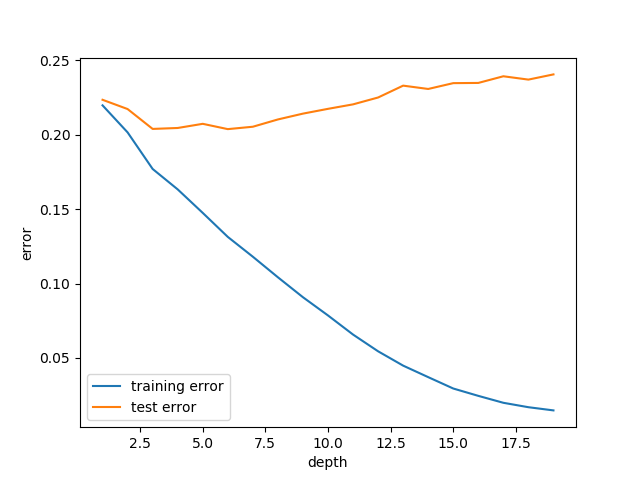
\includegraphics[scale=0.5]{Figure_2}}
The best depth limit to use for this data is data is a depth between 3 and 5. I notice that the test error in the graph is the lowest between 3 to 5 before the data starts to suffer from overfitting. I notice the overfitting the graph. From the graph we see that the training error decreases, but the test error increases. This means that the model is over fit to the test data because it can predict the labels of the test data with decreasing error, but when run on a test data set the model is unable to predict the labels correctly. 

\item Problem 4h \\
\solution{} \\
From the code, I obtained the following graph: \\
\centerline{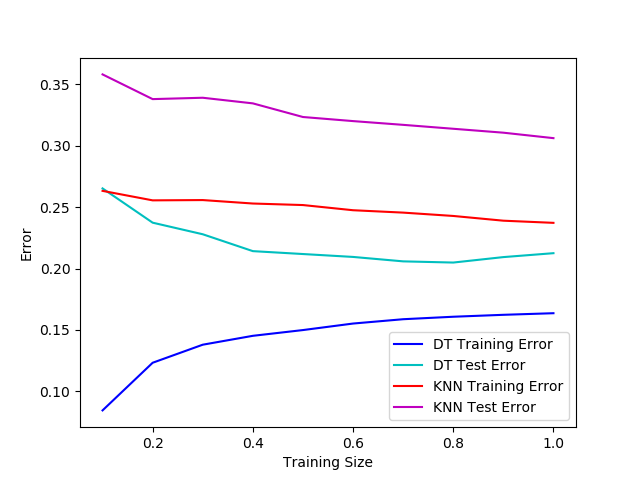
\includegraphics[scale=0.5]{Figure_3}}
For this graph, I used a depth of 4 for my decision tree and a k of 7 for my KNN. I noticed that the overall error for the DecisionTreeClassifier is lower than that of the KNeighborsClassifier. This analysis means that the DecisionTreeClassifier is a better model to use in this case than the KNeighborsClassifier. I also noticed that as the training size increased the DecisionTreeClassifier training and test error appeared to converged. From this we can conclude that the DecisionTreeClassifier is learning well because the test error is decreasing and we are making more accurate predictions on it.

The KNeighborsClassifier appeared to also improve with a larger training set. I think that this is because with a larger sample  space, the KNeighborsClassifier is able to make a more accurate prediction from its neighbors.
\end{enumerate}
\end{document}
